\section{AccSim Design Framework} \label{sec:customization-framework}
In this work, a flexible accelerator simulator framework AccSim is developed for 
rapid accelerator design and exploration. The framework overview and 
supported features will be presented in the following subsections.

\subsection{AccSim Overview}
AccSim overview is shown in \figref{fig:simframework}. It can be seen that 
an accelerator simulator roughly consists of user logic descrbing the application 
and memory models simulating the memory access. 

\begin{figure}[htb]
	\centering
	\label{fig:simframework}
	\caption{AccSim Framework}
	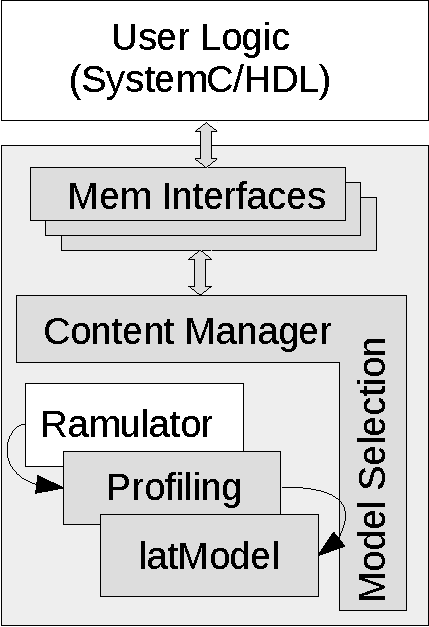
\includegraphics[width=.45\linewidth]{simframework}
\end{figure}



\subsection{Major AccSim Features}
memory interfaces

content management

co-simulation

simulation precision and speed trade-off


